\documentclass[12p,a4paper]{article}
\usepackage[utf8]{inputenc}
\usepackage[T1]{fontenc,url}
\usepackage{multicol}
\usepackage{multirow}
\usepackage{parskip}
\usepackage{lmodern}
\usepackage{microtype}
\usepackage{verbatim}
\usepackage{amsmath, amssymb}
\usepackage{tikz}
\usepackage{physics}
\usepackage{mathtools}
\usepackage{algorithm}
\usepackage{algpseudocode}
\usepackage{listings}
\usepackage{enumerate}
\usepackage{graphicx}
\usepackage{float}
\usepackage{hyperref}
\usepackage{tabularx}
\usepackage{siunitx}
\usepackage{fancyvrb}
\usepackage[makeroom]{cancel}
\usepackage[margin=3cm]{geometry}
\renewcommand{\baselinestretch}{1}
\setlength\parindent{0pt}


\begin{document}

\section*{Part 1 - The Einstein Crystal}

We will be looking at the 2 dimensional Einsten crystal, which is a grid of oscilating atoms with harmonic potential energy in each dimension. We will quantify the allowed energies in each oscilating direction, giving us $N$ oscilators with individual energy-levels $n_i$. We introduce a dimensionsless variable $q$ as the total energy-quantity of the system, $q = \sum n_i$.  We can extract the actual energy of the system as the energy-quantity times some scaling factor: $U = \epsilon q$.

\subsection*{Task a)}
Considering first a single Einstein crystal, with $N = 3$ oscilators, and energy $q=3$. The number of ways we can arrange these energies among the operators, is 10, as shown below.

\begin{tabular}{c|c c c}
    \textbf{Oscilator} $i$	& \textbf{1} & \textbf{2} & \textbf{3}\\
    \hline
    \multirow{10}{*}{\textbf{Energy} $n_i$}
                    & 0 & 0 & 3\\
     				& 0 & 1 & 2\\
     				& 0 & 2 & 1\\
     				& 0 & 3 & 0\\
     				& 1 & 0 & 2\\
     				& 1 & 1 & 1\\
     				& 1 & 2 & 0\\
     				& 2 & 0 & 1\\
     				& 2 & 1 & 0\\
     				& 3 & 0 & 0\\
\end{tabular}




\subsection*{Task b)}

\begin{align*}
    \Omega(N, q) &= \binom{q + N - 1}{q} = \frac{(q+N-1)!}{q!(N-1)!} \\
    \\
    \Omega(3, 3) &= \frac{(3+3-1)!}{3!(3-1)!} = \frac{5!}{3!2!} = \frac{5\cdot 4}{2} = 10
\end{align*}



\subsection*{Task c)}
We are now considering two Einstein crystals of $N_A = 2$ and $N_B=2$ oscilators, with $q_A=5$ and $q_B = 2$ energies at their disposal. While the two systems are unable to share energy, we see that there are a total of 15 possible microstates:

\begin{tabular}{c | c c | c c}
    \multicolumn{1}{c|}{} & \multicolumn{2}{c|}{\textbf{System A}} & \multicolumn{2}{c}{\textbf{System B}} \\
    \textbf{Oscilator} $i$
                    & \textbf{1} & \textbf{2} & \textbf{3} & \textbf{4}\\
    \hline
    \multirow{15}{*}{\textbf{Energy} $n_i$}
                    & 0 & 4 & 0 & 2 \\
     				& 1 & 3 & 0 & 2 \\
     				& 2 & 2 & 0 & 2 \\
     				& 3 & 1 & 0 & 2 \\
     				& 4 & 0 & 0 & 2 \\
     				& 0 & 4 & 1 & 1 \\
     				& 1 & 3 & 1 & 1 \\
     				& 2 & 2 & 1 & 1 \\
     				& 3 & 1 & 1 & 1 \\
     				& 4 & 0 & 1 & 1 \\
     				& 0 & 4 & 2 & 0 \\
     				& 1 & 3 & 2 & 0 \\
     				& 2 & 2 & 2 & 0 \\
     				& 3 & 1 & 2 & 0 \\
     				& 4 & 0 & 2 & 0 \\
\end{tabular}


\subsection*{Task d)}
Looking at the macrostates, there are a total of 7 ways we can distribute $q = q_A + q_B = 6$ quantities of energy, as shown below.

\begin{tabular}{c | c c}
    	& $q_A$ & $q_B$ \\
    \hline
    	&  0  &  6 \\
    	&  1  &  5 \\
    	&  2  &  4 \\
    	&  3  &  3 \\
    	&  4  &  2 \\
    	&  5  &  1 \\
    	&  6  &  0 \\
\end{tabular}


\subsection*{Task e)}
A given macrostate $q_A$ gives the following number of microstates in the system $N_A$:
\[
	\Omega(N_A,q_A) = \binom{q_A+N_A-1}{q_A} = \frac{(q_A+N_A-1)!}{q_A!(N_A-1)!}
\]
and the following number of microstates for $N_B$:
\[
	\Omega(N_B,q_B) = \binom{q_B+N_B-1}{q_B} = \frac{(q_B+N_B-1)!}{q_B!(N_B-1)!}
\]
This gives the total number of combination for the combined system as
\[
	\Omega(N, q) = \Omega(N_A,q_A)\Omega(N_B,q_B)
\]

If we apply this to the system $N_A=2$, $N_B=2$, $q=6$, we get

\[
	\Omega(4, 6) = \Omega(2,q_A)\Omega(2,q_B)
\]

The probability of getting a state $q_A$ is simply
\begin{align*}
    P(q_A) = \frac{\Omega(q_A)}{\Omega_{tot}}
\end{align*}


\begin{tabular}{c c c c c | c | c}
				& $q_A$ & $\Omega_A$ & $q_B$ & $\Omega_B$ & $\Omega=\Omega_A\Omega_B$ & $P(q_A) = \Omega/\Omega_{tot}$ \\
\hline
				& 0 & 1 & 6 & 7 & 7  & $8.3\%$\\
 				& 1 & 2 & 5 & 6 & 12 & $14.3\%$\\
 				& 2 & 3 & 4 & 5 & 15 & $17.9\%$\\
 				& 3 & 4 & 3 & 4 & 16 & $19\%$\\
 				& 4 & 5 & 2 & 3 & 15 & $17.9\%$\\
 				& 5 & 6 & 1 & 2 & 12 & $14.3\%$\\
 				& 6 & 7 & 0 & 1 & 7  & $9.3\%$\\
\hline
				&   &   &   &   & $\Omega_{tot}=84$ &
\end{tabular}
\\
\\

This corresponds with the output of our program (see apendix):\\

\lstinputlisting[frame=single]{task_e.dat}


\subsection*{Task f)}
We observe that the total number of microstates significantly increases when the systems are set in thermal contact. This is due to the higher number of possible combitations achived when all the 6 energy-levels are available to both the systems. From the table above, we can observe that our system $q_A = 4$ and $q_B = 2$ from task c) is simply a special case of a system where the energies are distributed freely among the two systems. The less constraints we put on our system, the more microstates becomes avaliable.



\subsection*{Task g)}

\begin{figure}[H]
    \centering
    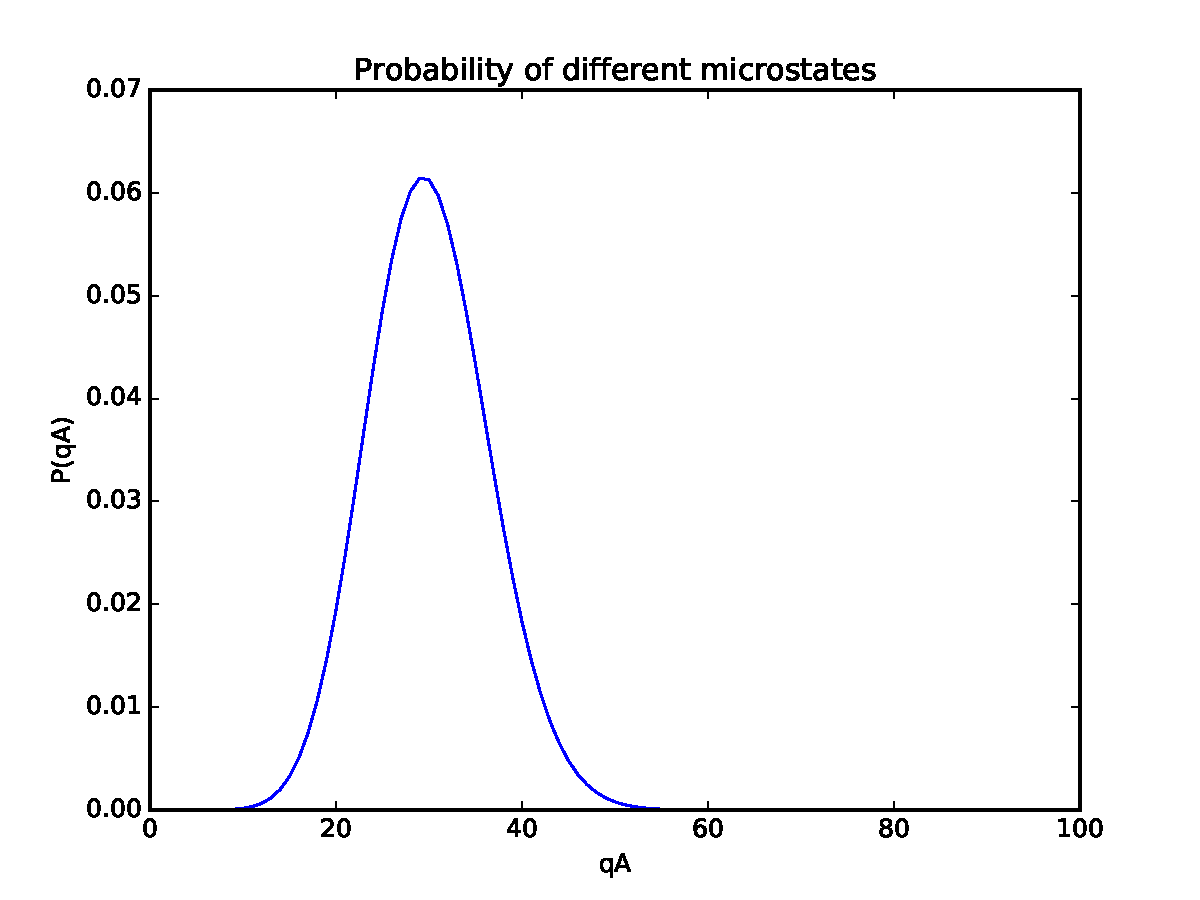
\includegraphics[scale=0.6]{task_g.pdf}
    \caption{asdf}
    \label{asdf}
\end{figure}


\subsection*{Task h)}
For large numbers $N$ and $q$, we are allowed to make the approximation
\begin{align*}
	\ln \Omega(N,q) = \ln \frac{(q+N-1)!}{q!(N-1)!} \approx \ln \frac{(q+N)!}{q!N!} \\
\end{align*}

Using the rules for logarithms, we can expand this to
\begin{align*}
    = \ln[(q+N)!] - \ln[q!] - \ln[N!]
\end{align*}

Using stirling approximation $\ln[x!] \approx x\ln[x] - x$, we get
\begin{align*}
    &\approx (q+N) \ln[q+N] -q -N -q\ln[q] +q -N\ln[N] + N \\
    &= (q+N)\ln[q+N] - q\ln[q] - N\ln[N] \\
    &= q\ln\qty[\frac{q+N}{q}] + N\ln\qty[\frac{q+N}{N}]
    = q\ln\qty[{1+\frac{N}{q}}] + N\ln\qty[\frac{q}{N}+1]
\end{align*}

Using the approximation $\ln[1+x] \approx x,\ x\ll 1$\footnote{A first order taylor expansion around $\ln[1]$ gives $\ln[1+x] = 0 + x + \mathcal{O}(x^2)$}, and taking into consideration that $q/N \gg 1$, we get

\begin{align*}
    \approx q\frac{N}{q} + N\ln\qty[\frac{q}{N}] = N + N\ln\qty[\frac{q}{N}] = N(\ln\qty[\frac{q}{N}] + 1)
\end{align*}

Giving the final result
\begin{align}\label{eqn:ln_omega}
     \ln \Omega(N,q) \approx N\qty(\ln\qty[\frac{q}{N}] + 1)
\end{align}


Or, a bit more generally, that
\begin{align}\label{eqn:binom_approx}
    \ln\binom{x+X}{x} = \frac{(x+X)!}{x!X!} \approx X\qty(\ln\qty[\frac{x}{X}] + 1)
\end{align}
for $x \gg 1$ and $x/X \gg 1$.




\subsection*{Task i)}
The definition of entropy is given as
\begin{align*}
    S = k\ln\qty[\Omega(N,q)]
\end{align*}

For a large Einstein crystal $N \gg 1$, with high energy $q \gg N$, we can use our approximation from equation \ref{eqn:ln_omega} to calculate the entropy:
\begin{align}\label{eqn:S}
    S = kN(\ln\qty[\frac{q}{N}] + 1)
\end{align}




\subsection*{Task j)}
The temperature of a system with an energy $U$ and entropy $S$ is given as
\begin{align*}
    \frac{1}{T} = \qty(\frac{\partial S}{\partial U})
\end{align*}

We can model the energy as a constant times our arbritrary quantified energy, $q$, giving $U = \epsilon q$.

We insert the expression \ref{eqn:S} for the Einstein crystals entropy into the derivative
\begin{align*}
    \frac{1}{T} &= \frac{\partial}{\partial q}\qty( kN(\ln\qty[\frac{U/\epsilon}{N}] + 1) )
                 = kN\frac{\partial}{\partial q}\qty( \ln\qty[\frac{U}{\epsilon N}] ) \\
                &= kN \qty(\frac{1}{\epsilon N} \frac{1}{\frac{q}{\epsilon N}} )
                 = k\frac{N}{U} \\
                T &= \frac{U}{kN}
\end{align*}

We see that we have a linear relation between temperature, total energy, and number of particles. This is as expected: If we double the energy, the temperature doubles, if we double the amount of particles while the energy stays the same, the temperature halves. If we add a bunch of particles with the same energy, the total energy and particles scales linearly, and the temperature stays the same. This all makes intuitive sense.

We can also solve for energy, and see that
\begin{align*}
    U = NkT = 2\cdot N\cdot \frac{1}{2}kT
\end{align*}
which according to the equipartition theorem corresponds to the energy of a system with two degrees of freedom. These degrees of freedom are the two velocity dimensions in our Einstein model.


\subsection*{Task k)}
Since each spin is binary, we can easially identify a combination of spins as a binary string of zeros and ones. Say, for instance, that we have 4 spins, +1, -1, -1, +1. We will write this as 1001, and can then treat this as a number in base 2. In base 10, this is 9. This way we can orderly represent each microstate of N particle as a number $< 2^N$. In a numerical approach, we would probably represent the spin system as a binary array of zeroes and ones.

Since every particle can be in two different spins, independently of each other, the total number of microstates becomes
\begin{align*}
    \Omega = 2^N
\end{align*}


\subsection*{Task l)}
\begin{align*}
    E_{tot} = -S_+\mu B + S_-\mu B = (S_- - S_+)\mu B = -s\mu B
\end{align*}




\subsection*{Task m)}
\begin{figure}[H]
  \centering
  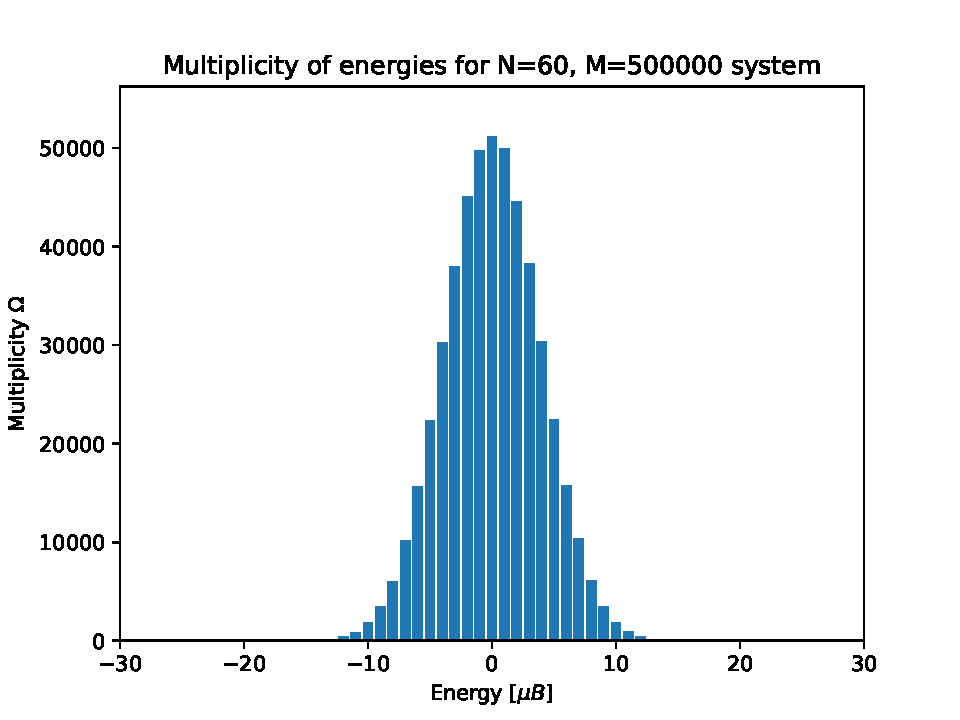
\includegraphics[scale=0.6]{task_m.pdf}
\end{figure}




\subsection*{Task n)}
For a given macrostate $S_+$, the multiplicity corresponds to the number of unique ways we can arrange $N = S_+ + S_-$ spins. There are $N!$ ways we can arrange a set of $N$ spins. But since we can't tell each individual spin up or spin down from one another, a lot of our configurations are identical. There are $S_+!$ ways of rearranging the up spins without making a difference, and $S_-!$ ways of doing the same for the down spins. There is therefore $S_+!S_-!$ ways of rearranging our spin configuration without changing it. The total number of unique configurations then become

\begin{align*}
  \Omega(N, S_+) = \frac{N!}{S_+!S_-!}
\end{align*}

We can also observe that this corresponds to
\begin{align*}
  \Omega(N, S_+) = \frac{N!}{S_+!S_-!} = \frac{N!}{S_+!(N-S_+)!} = \binom{N}{S_+}
\end{align*}
which we recognize as the number of ways of picking $S_+$ items out of a pool of $N$, or the number of ways of arranging $S_+$ and $N-S_+$ items.\footnote{These two cases are identical, if you imagine "picking $S_+$ items" as an action that turns those items from spin down to spin up.}




\subsection*{Task o)}
\begin{align*}
  S_+ &= S_- + 2s = N - S_+ + 2s \\
  S_+ &= \frac{N}{2} + s \\
\end{align*}
\begin{align*}
  S_- &= S_+ - 2s = N - S_- - 2s \\
  S_- &= \frac{N}{2} - s \\
\end{align*}
Giving
\begin{align*}
  \Omega(N, s) = \frac{N!}{S_+!S_-!} = \frac{N!}{\qty(\frac{N}{2} + s)!\qty(\frac{N}{2} - s)!}
\end{align*}


\subsection*{Task p)}
We know that the binomial distribution follows a gaussian curve, as
\begin{align*}
    \Omega(N,s) \approx \Omega_{max}e^{-2s^2/N}
\end{align*}


\subsection*{Task q)}
The analytical result corresponds great with our generated microstates.
\begin{figure}[H]
    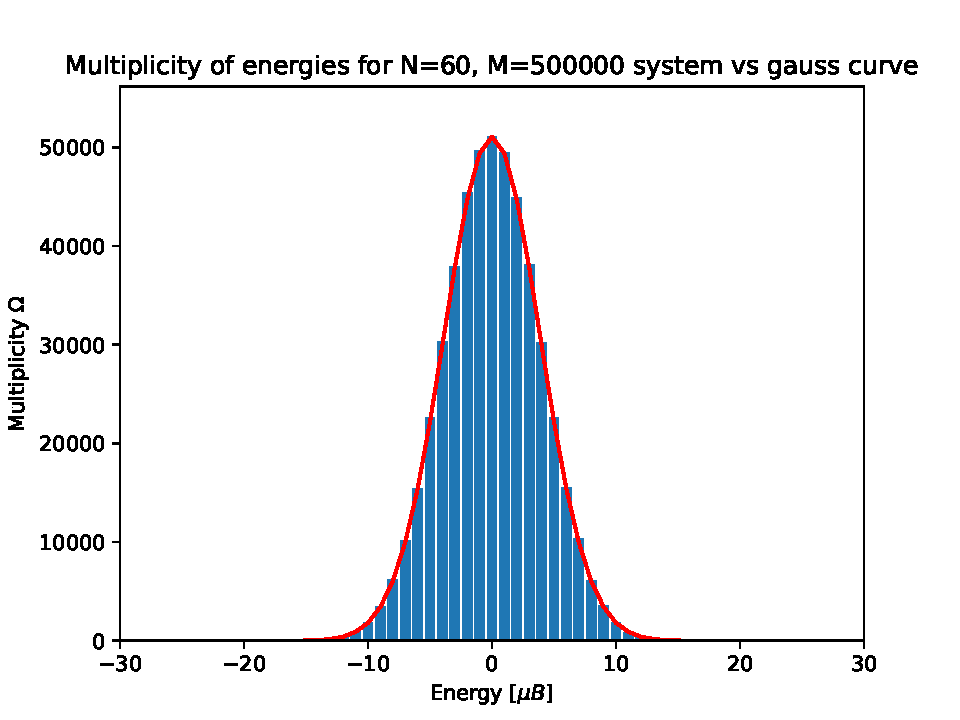
\includegraphics{task_q.pdf}
    \caption{}
    \label{}
\end{figure}

\subsection{Task r)}
We have the entropy defined as
\begin{align*}
    S = k\ln{Omega} = k\ln\qty(\frac{N!}{S_+!(N-S)!})
\end{align*}
We use stirlings approximation to get
\begin{align*}
    S \approx k N \ln N - S_+ \ln S_+ - (N-S_+)\ln(N-S_+)
\end{align*}

\subsection{Task s)}
We use the definition of temperature:
\begin{align*}
    \frac{1}{T} = \qty(\frac{\partial S}{\partial U}) = \frac{\partial S_+}{\partial U}\frac{\partial S}\partial{S_+} = -\frac{1}{2\mu B}\frac{\partial S}{\partial S_+}
\end{align*}


\end{document}
